\section{Contact Angle, Curvature, Bernoulli Condition}
\subsection{Contact Angle}
\hspace{0em}\indent Consider a droplet and a solid plane; the contact angle is the exterior angle between the two, as angle $\theta$ in Figure \ref{fig:cangle}. The contact angle indicates the hydrophilicity of the solid. 
\begin{figure}[H]
    \centering
    \adjustbox{frame=.25pt,frame,margin=.1pt,color=mycolor}{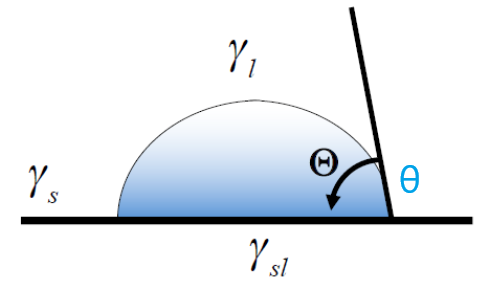
\includegraphics[width=0.45\linewidth]{Figs/young angle whole e.png}}\hspace{0.1em}
    \adjustbox{frame=.25pt,frame,margin=.1pt,color=mycolor}{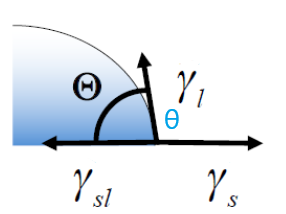
\includegraphics[width=0.35\linewidth]{Figs/young angle local e.png}} % Side by side images
    
    \caption{\small The left figure shows the global view of the contact angle, and the right figure shows its local scope. Here $\gamma_{s}$, $\gamma_{sl}$, and $\gamma_{l}$ are the surface tensions of the solid/gas, solid/liquid, and gas/liquid interfaces. For the static study, more complicated physical activities, such as hysteresis, are disregarded.}
    \label{fig:cangle}
\end{figure}
When the droplet is stabilized, the total force is zero. Thus, in the direction along the plane, we have \citeauthor{young_1805}'s equation:
\vspace{-1.em}
\begin{equation}\label{eqn:young}
    \gamma_{vl} \cos \theta_{eq} = \gamma_{s} - \gamma_{sl}\vspace{-1.em}
\end{equation}
Named after British scientist Thomas Young, it describes an equilibrium condition at the contact point of a droplet, solid surface, and another medium. 

From the energy perspective, consider only the plane of solid material in contact with air. The surface energy within contact area \(A\) is:
%\vspace{-1.em}
\[
E_1=\gamma_{s}\, A%\vspace{-1.em}
\]
$\gamma\coloneqq F/L$ is the surface tension. In $\mathbb{R}^3$, $[\gamma]=N/m$ and $[\gamma A]=J$ . When a droplet occupies area \(A\) in contact with the solid, and contacts air over an area \(A_{vl}\), the corresponding energy is
\[E_2=\gamma_{sl} A + \gamma_{vl} A_{vl}\]
Neglecting gravity, the droplet will stabilize if the energy difference is minimized\footnote{This principle is discussed in \citet{Gibbs1878}.}, rather than minimizing \(E_2\), leading to Young's equation (\ref{eqn:young}).
\[0\equiv\Delta E = E_2-E_1=(\gamma_{sl}-\gamma_{s})A+\gamma_{vl}A_{vl}\]
The boundary of the droplet tends to shrink, while the volume of the droplet is constant. In the complete wetting case, $A=A_{vl}$, $\theta_{eq}=0\degree$, the liquid covers the solid surface as much as possible. 
\[\Delta E = E_2-E_1=\left[(\gamma_{sl}-\gamma_{s})+\gamma_{vl}\right]A\]
In the $\theta_{eq}=\pi/2$ case, the equation becomes $\gamma_{sl}=\gamma_s$.

When an external voltage is applied, the corresponding contact angle is experimentally found to be a function of the voltage difference between the droplet and the surroundings, the capacitance of the involved dielectric, and the surface tension of the droplet.
\[\cos \theta_Y = \cos \theta + \frac{C}{2 \gamma} U^2\]

\subsection{The Mean Curvature and Normal Stress}
\hspace{0em}\indent The (mean) curvature\footnote{One of the definitions is the divergence of the normal direction of a curve \( f(\vec{r}) \):
\[ \kappa \coloneqq \nabla \cdot \frac{\nabla f}{|\nabla f|} \]} measures the normal displacement as the surface or line extends. For a length extension \(\Delta L\) along the curve, the increase in the normal direction is \( \kappa \Delta L \).

Consider a material with a continuous boundary surface in $\mathbb{R}^3$ or a boundary line in $\mathbb{R}^2$. The normal stress per unit length due to curvature, is the force in the normal direction along the curve per unit length caused by surface tension:
\[
\vec{F}_{\gamma}=\gamma \kappa\hat{n}
\]
\subsection{Bernoulli Condition with Curvature}
Bernoulli Condition
\[
P+\frac{1}{2}\rho v^2+\rho g h = Cst\hspace{0.5em},\hspace{1em}\text{on a streamline}
\]
With curvature, the pressure difference at points on the streamline is 
\begin{equation}
    \Delta p =\gamma \kappa\label{Delta_P}
\end{equation}
Let $g=0$, and pick point 1 as a reference and random point 2 on the streamline, 
\[\frac{P_1}{\rho}+\frac{1}{2}v_1^2=\frac{P_2}{\rho}+\frac{1}{2}v_2^2=Cst\Longrightarrow \frac{\gamma K}{\rho}+\frac{1}{2}v_2^2=\frac{1}{2}v_1^2 =Cst_1\]
This corresponds to the non-dimensionalised form of equation (10), \citet{Crowdy2015} and equation (1.6), \citet{Fontelos2008_2}, in the presence of electric effect:
\begin{equation}\label{boundary_k}
\kappa-\left|\frac{\df w(z)}{\df z}\right|^2=Cst    
\end{equation}